\section{Specification}
We utilize Chisel(Constructing Hardware In a Scala Embedded
Language)~\cite{Bachrach:2012} as the basis of our datapath and
pipelining specification. Chisel is an experimental hardware
description language implemented through a set of class definitions
within the high level programming language Scala. Chisel allows for
the designer to fully leverage the high level object oriented
programming features of the Scala language to succinctly describe
hardware. A design described in Chisel can be mapped to a C++
simulator or Verilog emitted for either FPGA simulation or ASIC
synthesis.

\subsection{Datapath Specification}
The datapath can be specified by a set of architectural state elements
and their next state update logic. We also add a special {\tt Variable
Latency Interface} to allow users to integrate into the datapath
functional units that do not have valid output available every cycle,
such as caches and multi-cycle dividers. In the context of our
specification, Chisel's existing syntax is used to wire up
combinational logic and modules implementing the Variable Latency
Interface, which functions as next state logic, to Reg and Transaction
Mem constructs, which function as a single architectural state element
and an addressable array of architectural state respectively.

{\bf Regs}. {\tt Regs} are existing Chisel constructs that represent a
single multi-bit wide flip-flop with synchronous reset and clock
enable ports. They can be treated as single piece of architectural
state that is conditionally updated by every transaction contingent on
the clock enable input.

\begin{figure}[htb]
\centering
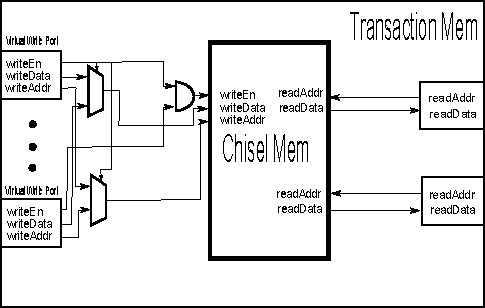
\includegraphics{figures/TMEM.pdf}
\caption{{\bf Transaction Mem} Shows an example of a Transaction Mem with many virtual write ports, one physical write port, and two read ports}
\label{fig:tmem}
\end{figure}

{\bf Transaction Mems}. Transaction Mems are Chisel Components that
wrap existing Chisel Mem constructs in an IO interface that helps the
automatic synthesis tools detect bypassing opportunities. On
instantiation the {\tt Transaction Mem} allows the user to specify the
number of lines in the memory, number of read ports on the IO, number
of virtual write ports on the IO, and the number of physical write
ports on the underlining Chisel Mem construct. Each read port consists
of a read address input and a read data output. There is a one to one
mapping between {\tt Transaction Mem} read ports and underlining read ports
in the Chisel Mem construct. Each virtual write port consists of a
write address input, write enable input, and write data input. The
{\tt Transaction Mem} wrapper automatically maps the virtual write ports on
the IO to the physical write ports of the underlining Chisel Mem
construct. If the number of virtual write ports exceeds the number of
physical write ports, the {\tt Transaction Mem} module automatically
coalesces multiple virtual write ports onto a single physical write
port by muxing together the write data and write addresses of the
virtual write ports and ORing together the write enables of the
virtual write ports. The user should wire each distinct source of
write data along with the associated write enable and write address
into separate virtual write ports rather than manually coalescing the
write data together with a mux and wiring the output of the mux into
a single virtual write port in order to allow the automatic synthesis
tools to generate fine grained bypass logic. This will be elaborated
upon in 4.3.
\begin{figure}[htb]
\centering
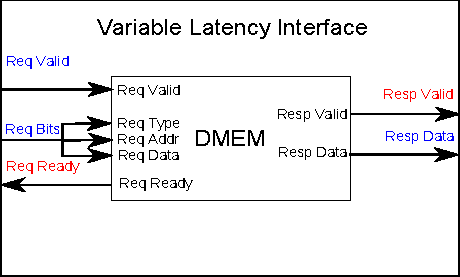
\includegraphics{figures/VLI.pdf}
\caption{{\bf Variable Latency Interface} Blue wires are user facing IO and read wires are tool facing IO.}
\label{fig:vli}
\end{figure}

{\bf Variable Latency Interface}. Variable latency Interfaces are a
Chisel Components that specify a set of user facing IO to allow users
to integrate an existing variable/multi-cycle latency Chisel module
into the datapath specification and a set of tool facing IO to allow
the automatic synthesis tools to generate appropriate pipeline logic
to deal with variable/multi-cycle latency modules. The Variable
Latency Interface exposes on its user facing IO a request ready input,
request data input, and response data output. The user connects the
user facing IO to the rest of the datapath using standard Chisel
syntax. The tool facing IO includes a request ready output and a
response valid output. The tools use the request ready output to
generate logic that puts back pressure on the pipeline stages before
the variable latency module and use the response valid output to
generate logic to insert bubbles into the pipeline stages after the
variable latency module. Figure~\ref{fig:vli}gives and example of how to
integrate a Data Cache into the datapath specification through
wrapping it in a Variable Latency Interface.

Everything used in the datapath specification is either a built in
Chisel construct(Regs and combinational logic) or a ordinary Chisel
Component(TransactonMems and Variable Latency Module Interfaces). This
allows the user to create a datapath specification in the exact same
way they would write an ordinary Chisel module, with the exception
that they have to use TransactionalMems in place of Mem constructs and
have to wrap up functional units that do not have valid output data
every cycle in Variable Latency Interfaces. The datapath specification
by itself, without any pipelining specification, functions as a single
cycle implementation of the datapath.

\subsection {Pipelining Specification}
Once the single cycle datapath has been specified, the user can add
separate annotations to specify how the datapath should be
pipelined. The main parameters in pipelining specification is the
placement of the pipeline registers, the depth of the pipeline, and
how pipeline hazards are resolved.

{\bf Pipeline register placement}. The placement of the pipeline
registers is specified by annotating combinational logic nodes and
read/write ports of the architectural state elements with pipeline
stage numbers. The user can annotate just the big pieces of combinational
logic and architectural state they care about, such as ALUs, register
files, or caches, and the automatic synthesis tool will infer the
placement of all the other parts of the datapath. Of course, the user
gains more control over the placement of the pipeline registers by
adding more pipeline stage annotations. The user can have complete
control over the placement of the pipeline registers if they annotate
every combinational logic node and read/write port in the datapath. The details of the pipeline
register placement are elaborated in section 4.1.

{\bf Pipeline depth}. Pipeline depth is inferred from the maximum
pipeline stage number the user annotates a combinational logic node or
read/write port with.


